\appendix
\chapter{Learned sensing matrices}
\subsection{Unsupervised alpha network}

Figure \ref{fig:Phial} shoes the graphical representation of the sensing matrix learned during training. Each small square is interpreted as the subsampling matrix for each input dimension.

\begin{figure}[!htb] 
\vspace{1cm}
\centering 
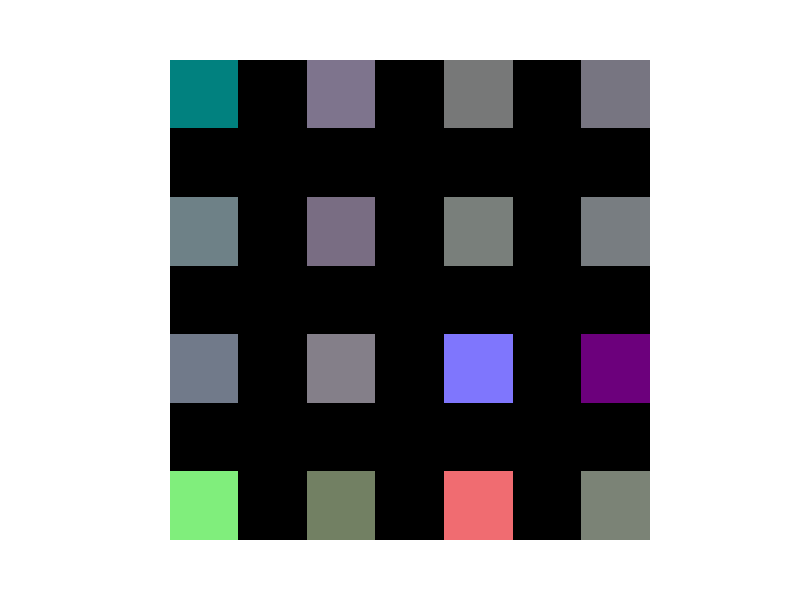
\includegraphics[width=\textwidth,height=\textheight,keepaspectratio=true]{Conv1alpha.png}
\caption[Learned sensing matrix for alpha network]{Sensing matrix for alpha network.}
\label{fig:Phial} 
\end{figure} 

\FloatBarrier

%\begin{table}[tb]
%\caption[Details of $\alpha$ Network]{Original features of each dataset.}
%\label{tab:AlphaNetpar}
%\centering
%\begin{tabular}{l*{6}{c}r}
%Number of layers & Size input layer & size output layer & Number of parameters $\omega$%\\
%\hline
%   &  &  &  &  \\
%\bottomrule 
%\end{tabular}  
%\end{table}

\subsection{Unsupervised beta network}

Figure \ref{fig:Phial} shoes the graphical representation of the sensing matrix learned during training. Each small square is interpreted as the subsampling matrix for each input dimension.

\begin{figure}[!htb] 
\vspace{1cm}
\centering 
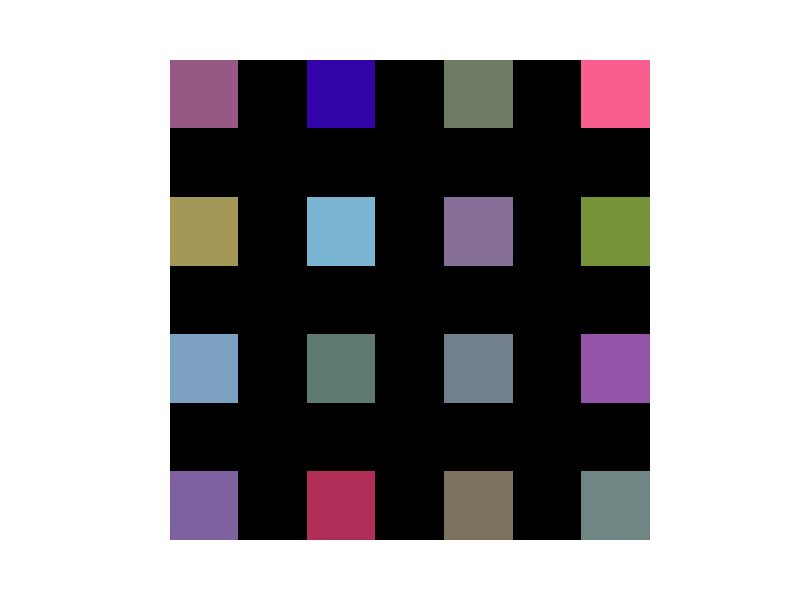
\includegraphics[width=\textwidth,height=\textheight,keepaspectratio=true]{Conv1beta.png}
\caption[Learned sensing matrix for alpha network]{Sensing matrix for beta network.}
\label{fig:Phial} 
\end{figure} 

\FloatBarrier

